% Options for packages loaded elsewhere
\PassOptionsToPackage{unicode}{hyperref}
\PassOptionsToPackage{hyphens}{url}
%
\documentclass[
]{article}
\usepackage{amsmath,amssymb}
\usepackage{lmodern}
\usepackage{iftex}
\ifPDFTeX
  \usepackage[T1]{fontenc}
  \usepackage[utf8]{inputenc}
  \usepackage{textcomp} % provide euro and other symbols
\else % if luatex or xetex
  \usepackage{unicode-math}
  \defaultfontfeatures{Scale=MatchLowercase}
  \defaultfontfeatures[\rmfamily]{Ligatures=TeX,Scale=1}
\fi
% Use upquote if available, for straight quotes in verbatim environments
\IfFileExists{upquote.sty}{\usepackage{upquote}}{}
\IfFileExists{microtype.sty}{% use microtype if available
  \usepackage[]{microtype}
  \UseMicrotypeSet[protrusion]{basicmath} % disable protrusion for tt fonts
}{}
\makeatletter
\@ifundefined{KOMAClassName}{% if non-KOMA class
  \IfFileExists{parskip.sty}{%
    \usepackage{parskip}
  }{% else
    \setlength{\parindent}{0pt}
    \setlength{\parskip}{6pt plus 2pt minus 1pt}}
}{% if KOMA class
  \KOMAoptions{parskip=half}}
\makeatother
\usepackage{xcolor}
\IfFileExists{xurl.sty}{\usepackage{xurl}}{} % add URL line breaks if available
\IfFileExists{bookmark.sty}{\usepackage{bookmark}}{\usepackage{hyperref}}
\hypersetup{
  pdftitle={Second task},
  pdfauthor={Akvilė Višniauskaitė ir Ieva Pudžiuvelytė},
  hidelinks,
  pdfcreator={LaTeX via pandoc}}
\urlstyle{same} % disable monospaced font for URLs
\usepackage[margin=1in]{geometry}
\usepackage{graphicx}
\makeatletter
\def\maxwidth{\ifdim\Gin@nat@width>\linewidth\linewidth\else\Gin@nat@width\fi}
\def\maxheight{\ifdim\Gin@nat@height>\textheight\textheight\else\Gin@nat@height\fi}
\makeatother
% Scale images if necessary, so that they will not overflow the page
% margins by default, and it is still possible to overwrite the defaults
% using explicit options in \includegraphics[width, height, ...]{}
\setkeys{Gin}{width=\maxwidth,height=\maxheight,keepaspectratio}
% Set default figure placement to htbp
\makeatletter
\def\fps@figure{htbp}
\makeatother
\setlength{\emergencystretch}{3em} % prevent overfull lines
\providecommand{\tightlist}{%
  \setlength{\itemsep}{0pt}\setlength{\parskip}{0pt}}
\setcounter{secnumdepth}{-\maxdimen} % remove section numbering
\newlength{\cslhangindent}
\setlength{\cslhangindent}{1.5em}
\newlength{\csllabelwidth}
\setlength{\csllabelwidth}{3em}
\newlength{\cslentryspacingunit} % times entry-spacing
\setlength{\cslentryspacingunit}{\parskip}
\newenvironment{CSLReferences}[2] % #1 hanging-ident, #2 entry spacing
 {% don't indent paragraphs
  \setlength{\parindent}{0pt}
  % turn on hanging indent if param 1 is 1
  \ifodd #1
  \let\oldpar\par
  \def\par{\hangindent=\cslhangindent\oldpar}
  \fi
  % set entry spacing
  \setlength{\parskip}{#2\cslentryspacingunit}
 }%
 {}
\usepackage{calc}
\newcommand{\CSLBlock}[1]{#1\hfill\break}
\newcommand{\CSLLeftMargin}[1]{\parbox[t]{\csllabelwidth}{#1}}
\newcommand{\CSLRightInline}[1]{\parbox[t]{\linewidth - \csllabelwidth}{#1}\break}
\newcommand{\CSLIndent}[1]{\hspace{\cslhangindent}#1}
\usepackage{float}
\ifLuaTeX
  \usepackage{selnolig}  % disable illegal ligatures
\fi

\title{Second task}
\author{Akvilė Višniauskaitė ir Ieva Pudžiuvelytė}
\date{4/22/2022}

\begin{document}
\maketitle

\hypertarget{introduction}{%
\section{Introduction}\label{introduction}}

This work will present data analysis from a research that studied the
enchancer's at \emph{IGF2} differential methylation association with
abnormal dopamine synthesis in major psychosis (Pai et al., 2019).

Our samples were taken from the prefrontal cortex isolated neurons from
patients with schizophrenia and bipolar disorder.

The study analysed data from individuals diagnosed with schizophrenia,
bipolar disorder, and controls (29, 26 and 27 individuals respectively).
In the analysis, study controlled for age, sex, post-mortem interval,
genetic ancestry (determined by genotyping the same individuals).

\hypertarget{experiment-design}{%
\subsection{Experiment design}\label{experiment-design}}

The experiment design was multi-omics study with 55 cases (with
schizophrenia or bipolar disorder) and 27 controls.

\hypertarget{objective-of-the-research}{%
\subsection{Objective of the research}\label{objective-of-the-research}}

According to authors, schizophrenia and bipolar disorder have got
characteristic of periods of psychosis. The main objective of the
research was to gather epigenomic profiling data to get a more accurate
model of neuronal dysregulation in diseases with periods of psychosis.

\hypertarget{biological-targets-of-the-research}{%
\subsection{Biological targets of the
research}\label{biological-targets-of-the-research}}

Researchers intended to look for specific patterns of DNA methylation in
isolated neurons from the frontal cortex of individuals that had
diseases.

\begin{itemize}
\tightlist
\item
  IGF2 - insulin growth factor 2 protein
\item
  \emph{IGF2} - IGF2 gene
\item
  \emph{Igf2} - enhancer of \emph{IGF2}
\item
  TH - tyrosine hydroxylase protein
\item
  dopamine - a neuromodulatory molecule
\item
  psychosis - an abnormal condition of the mind that results in
  difficulties determining what is real and what is not real
\end{itemize}

\hypertarget{results-received}{%
\subsection{Results received}\label{results-received}}

Authors found a strong association between methylation of \emph{Igf2}
and TH synthesis. TH is the bottleneck enzyme that is responsible for
dopamine synthesis. If enhancer \emph{Igf2} is hypomethylated, levels of
TH are higher, which determines the higher production of dopamine.
Apparently, dopamine is responsible for psychosis in the mental
disorders of interest.

\hypertarget{additional-information}{%
\subsection{Additional information}\label{additional-information}}

Schizophrenia and bipolar disorder patients are consistently
hypomethylated at \emph{IGF2} locus when compared to controls. This
locus remained significantly hypomethylated even after accounting
lifestyle-related variables of smoking and anti-psychotic use.

The reaction chain of interest of the research (upward arrows show
elevated expression or synthesis of the protein, product, or effect):

Hypomethylation of \emph{Igf2} \(\rightarrow\) \(\uparrow\) IGF2
\(\rightarrow\) \(\uparrow\) TH \(\rightarrow\) \(\uparrow\) dopamine
\(\rightarrow\) \(\uparrow\) psychosis

\hypertarget{data-preparation}{%
\section{Data preparation}\label{data-preparation}}

Sample keys heading is made of the following columns names:

\begin{itemize}
\tightlist
\item
  \emph{id} - an identifier of the sample
\item
  \emph{sentrix\_id} - Illumina's Sentrix BeadChip identifier (13 unique
  values) (National Institutes of Health, n.d.)
\item
  \emph{sentrix\_row} - row number in the Sentrix array
\item
  \emph{sentrix\_col} - column number in the Sentrix array
\item
  \emph{basename} - sample identifier in the research (joined values in
  a format:
  \newline [\textit{id}]\_{[}\emph{sentrix\_id}{]}\_R0{[}\emph{sentrix\_row}{]}C0{[}\emph{sentrix\_id}{]})
\item
  \emph{tissue\_bank\_id} - an identifying number of the tissue bank
  from which the sample was taken
\item
  \emph{tissue\_bank} - the literal identifier of the tissue bank
\item
  \emph{tissue} - a tissue type from which the sample was taken
\item
  \emph{cell\_type} - a cell type found in the sample
\item
  \emph{donor} - an integer number that identifies the donor of the
  sample (82 unique values)
\item
  \emph{pmi} - a post-mortem interval, unknown values were labeled as NA
\item
  \emph{race} - race of the donor (white, black, hispanic, or unknown
  (NA))
\item
  \emph{sex} - gender of the donor
\item
  \emph{diagnosis} - an experimental group of the donor (bipolar,
  schizophrenia, or control)
\item
  \emph{age} - age of the donor (years)
\end{itemize}

As it was noted in the article, there were 100 records in the sample
keys dataset.

\hypertarget{calculating-detection-p-values}{%
\subsection{Calculating detection
p-values}\label{calculating-detection-p-values}}

Getting detection p-value for each score of DNA modification. These
p-values determine whether the measured intensity can be distinguished
from the background.

All values that have got p-value higher than 0.01 are considered as bad
and all samples that have more than 1\% of bad detection p-values should
be removed.

Although, in our data, none of the samples had more than 1\% of bad
values, therefore no sample was removed.

\hypertarget{predicting-sample-sex}{%
\subsection{Predicting sample sex}\label{predicting-sample-sex}}

This stage estimates sample sex based on methylation data.

Number of females and males after estimation matched original data (25
female and 75 male).

Converted `M' and `F' notation to `male' and `female'.

No mismatches between real and estimated sex were found.

\hypertarget{data-normalisation}{%
\subsection{Data normalisation}\label{data-normalisation}}

According to the documentation of \emph{minfi} package (Fortin \&
Hansen, n.d.), \emph{preprocessFunnnorm()} function is recommended for
known large-scale differences (for example, cancer/normal) or
between-tissue studies. Our chosen data spans only over one cell type of
one tissue, therefore it was decided to opt for different normalisation
methods.

Authors (Pai et al., 2019) noted that they used noob normalisation
followed by the quantile one. Quantile normalisation performs processing
of Type I and Type II array design differences. Whereas,
\emph{preprocessIllumina()} normalisation has only background
subtraction and control normalisation implemented. Therefore, we decided
to choose \emph{preprocessSWAN()} normalisation, since this method
performs within-array normalisation correction for technical differences
between Type I and Type II array designs.

\hypertarget{filtering-position-data-by-detection-p-values}{%
\subsection{Filtering position data by detection
p-values}\label{filtering-position-data-by-detection-p-values}}

There were 5835 positions found that had p-value higher than 0.01 in 1\%
of the samples. These positions were removed from the dataset. After
this procedure, we have 861001 positions in each sample.

\hypertarget{removing-methylation-loci-positions}{%
\subsection{Removing methylation loci
positions}\label{removing-methylation-loci-positions}}

2918 methylation loci that do not contain ``CG'' nucleotide pair (CH
probes) or are close to DNR polymorphisms were removed. After the
removal data contained 858083 positions in each sample.

\hypertarget{making-three-different-data-objects}{%
\subsection{Making three different data
objects}\label{making-three-different-data-objects}}

The DNA modification score matrix was generated and was saved as well as
the information about main matrix samples and information about main
matrix positions into files for later manipulations with the data.

\pagebreak

\hypertarget{interarray-correlation-outliers-elimination}{%
\subsection{Interarray correlation outliers
elimination}\label{interarray-correlation-outliers-elimination}}

Identification and removal of samples with divergent modification
scores.

\begin{figure}[!h]
  \begin{center}
    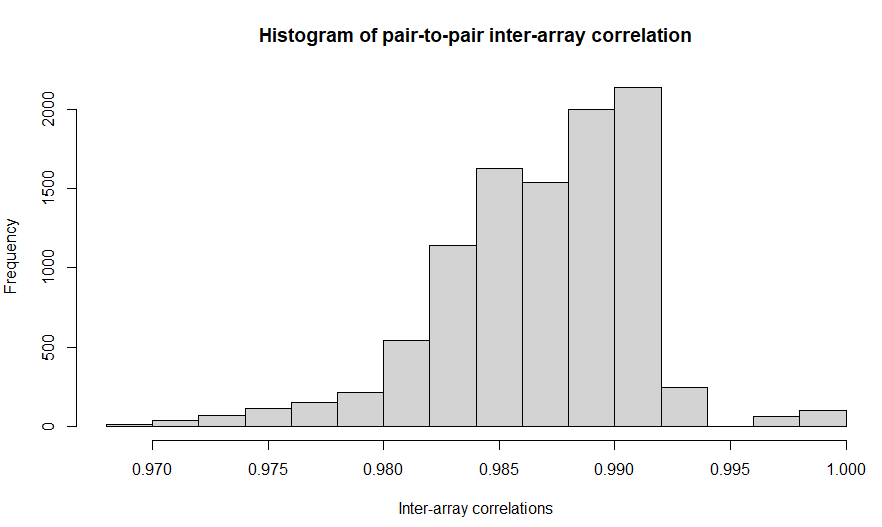
\includegraphics[width=75mm]{./1.png}
    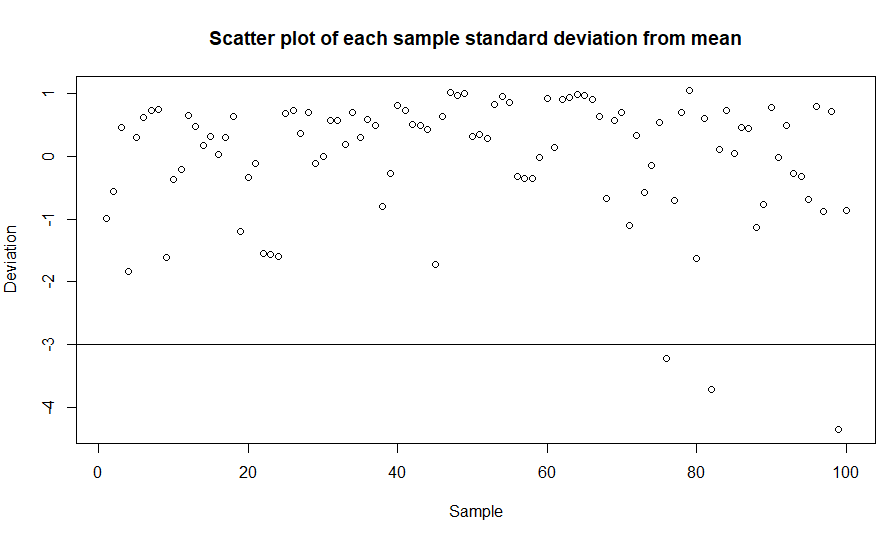
\includegraphics[width=75mm]{./2.png}
    \caption{
    The correlation histogram (left) and scatter plot (right) to detect the 
    outliers for elimination.
    }
  \end{center}
\end{figure}

The histogram (Figure 1) identifies that our dataset contains values
which distort the overall distribution. For further investigation,
standard deviation from mean in each sample was calculated.

Scatter plot of each sample (column) (Figure 1) standard deviation from
mean visually highlights the data outliers (under -3 limit of
deviation).

Algorithm identified and removed 3 outliers:

\begin{itemize}
\tightlist
\item
  GSM3059462\_200590490031\_R08C01 - a control sample of 53-year-old
  male
\item
  GSM3059520\_200357150067\_R08C01 - a sample of a 56-year-old male with
  bipolar disorder
\item
  GSM3059454\_200590490031\_R01C01 - a sample of a 77-year-old female
  with schizophrenia
\end{itemize}

\begin{figure}[!h]
  \begin{center}
    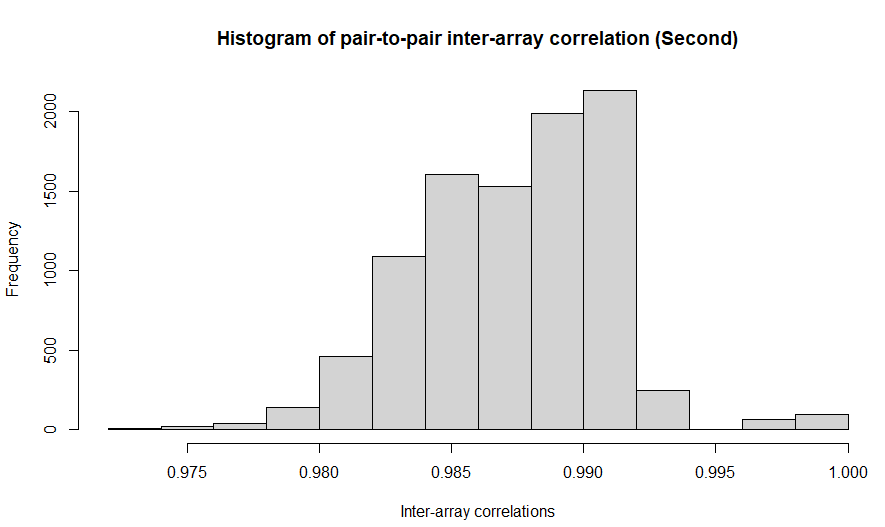
\includegraphics[width=75mm]{./3.png}
    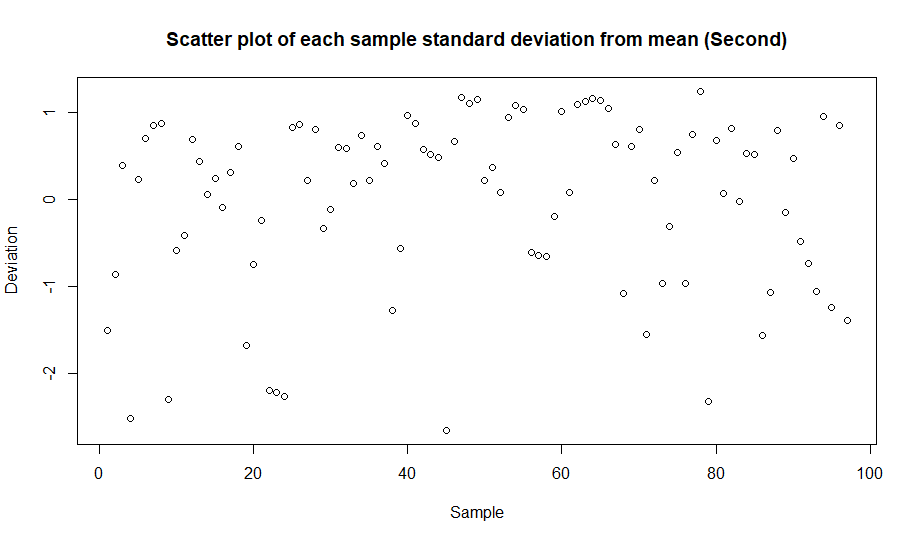
\includegraphics[width=75mm]{./4.png}
    \caption{
      The correlation histogram (left) and scatter plot (right) of all dataset 
      after the elimination of outliers.
    }
  \end{center}
\end{figure}

There is a visible difference on the left side of the histogram (Figure
2) compared to the histogram before the removal of outliers (Figure 1).
This change indicated that the distorting values were removed correctly.

No outliers were left in the recalculated scatter plot (Figure 2).

\newpage

\hypertarget{quality-control}{%
\subsection{Quality control}\label{quality-control}}

After all data manipulations, our set has 97 samples with 858083
positions.

Data for quality control was separated into case (65 samples) and
control (32 samples). Our main goal is to check if distortions in the
methylation data exist.

\begin{figure}[!h]
  \begin{center}
    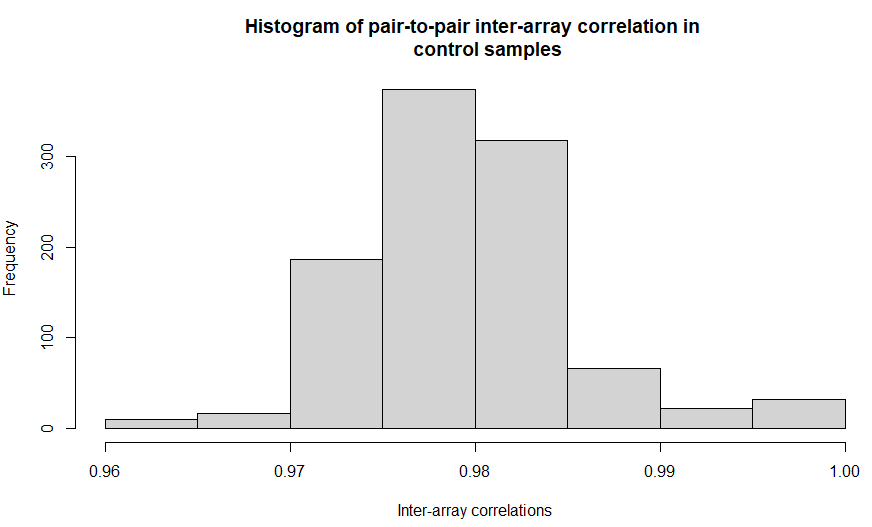
\includegraphics[width=75mm]{./5.png}
    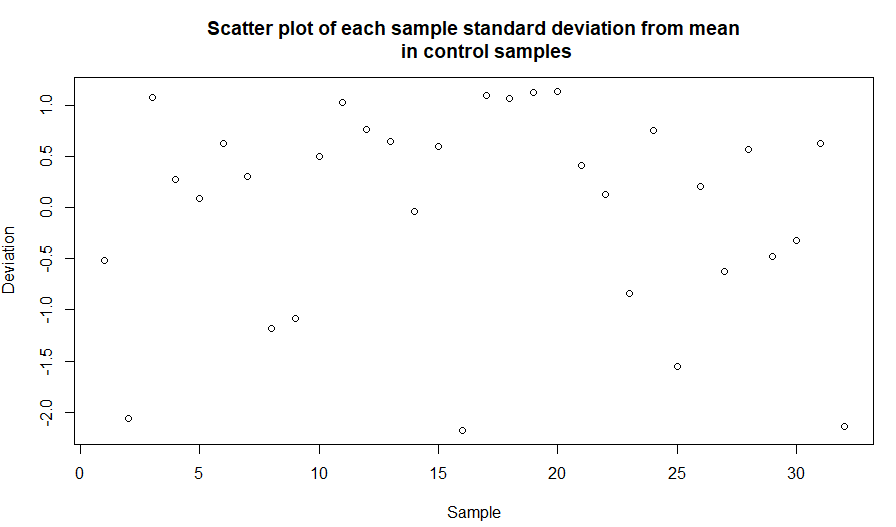
\includegraphics[width=75mm]{./7.png}
    \caption{
      The pair-to-pair correlation histogram (left) and scatter plot (right) for 
      control samples.
    }
  \end{center}
\end{figure}

The histogram (Figure 3) represents a pair-to-pair correlation in
control methylation data.

We can indicate both from histogram and scatter plot (Figure 3) that
data is distributed normally and there is no need for data removal.

Sequentially, it was decided to check the distribution of case
methylation data.

\begin{figure}[!h]
  \begin{center}
    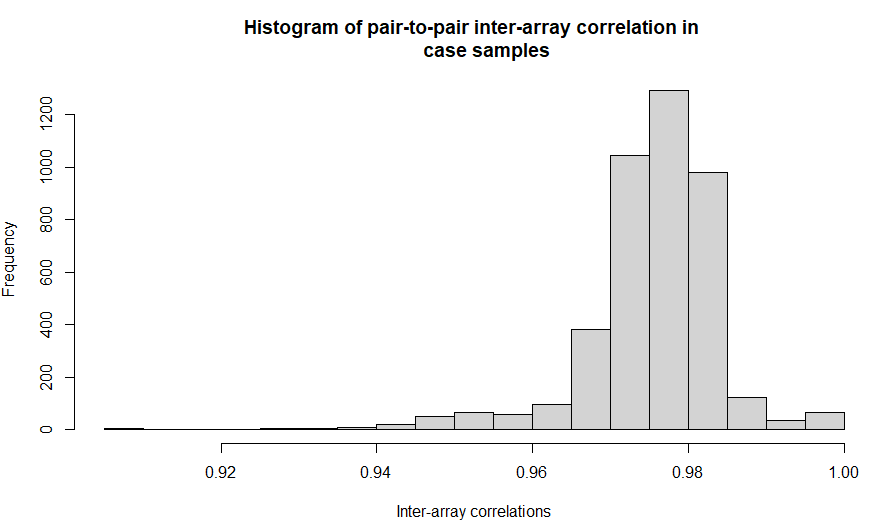
\includegraphics[width=75mm]{./6.png}
    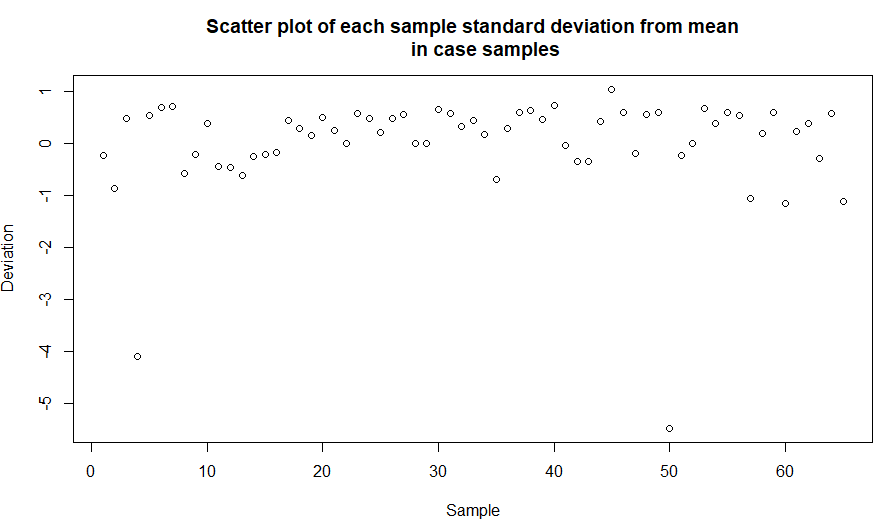
\includegraphics[width=75mm]{./8.png}
    \caption{
      The pair-to-pair correlation histogram (left) and scatter plot (right) of 
      all case samples.
    }
  \end{center}
\end{figure}

The scatter plot (Figure 4) of all case samples indicates, that our data
has distorted values in respect of all case samples mean. It
demonstrates two outliers in standard deviation from methylation mean.
For further analysis we separated case data into ``bipolar'' and
``schizophrenia'' cases.

\begin{figure}[!h]
  \begin{center}
    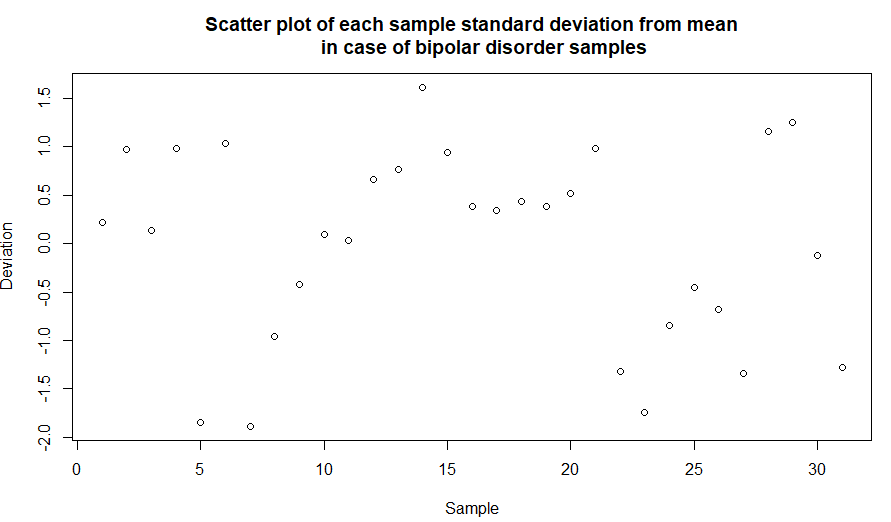
\includegraphics[width=90mm]{./9.png}
    \caption{
      The scatter plot of the bipolar samples.
    }
  \end{center}
\end{figure}

The scatter plot (Figure 5) with bipolar cases does not show any big
fluctuations from the mean methylation value of bipolar disorder case
samples.

\begin{figure}[!h]
  \begin{center}
    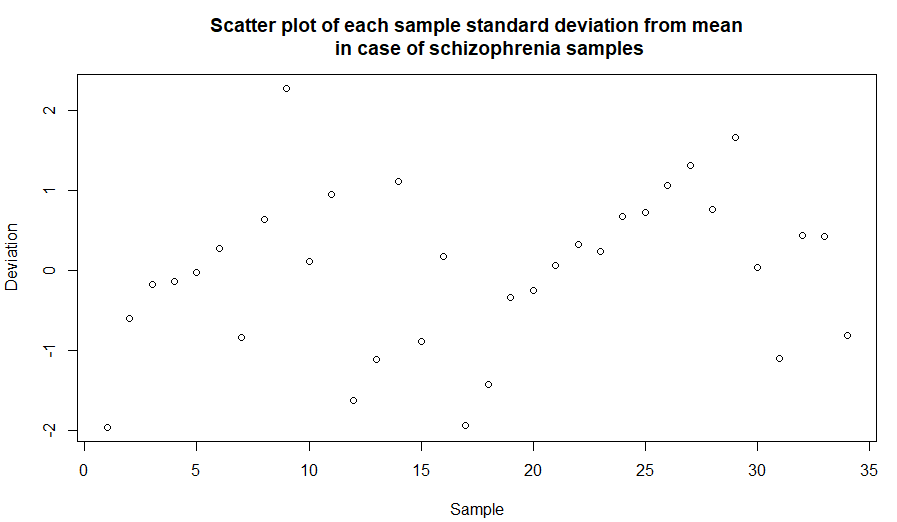
\includegraphics[width=90mm]{./10.png}
    \caption{
      The scatterplot of the schizophrenia case samples.
    }
  \end{center}
\end{figure}

The scatter plot (Figure 6) of schizophrenia cases also does not show
any wide variations from the mean methylation value.

These separated data cases indicated that there is no need to remove any
samples.

Additionally, the sample-specific quality control for methylation data
with getQC, addQC, and plotQC functions was estimated.

\begin{figure}[!h]
  \begin{center}
    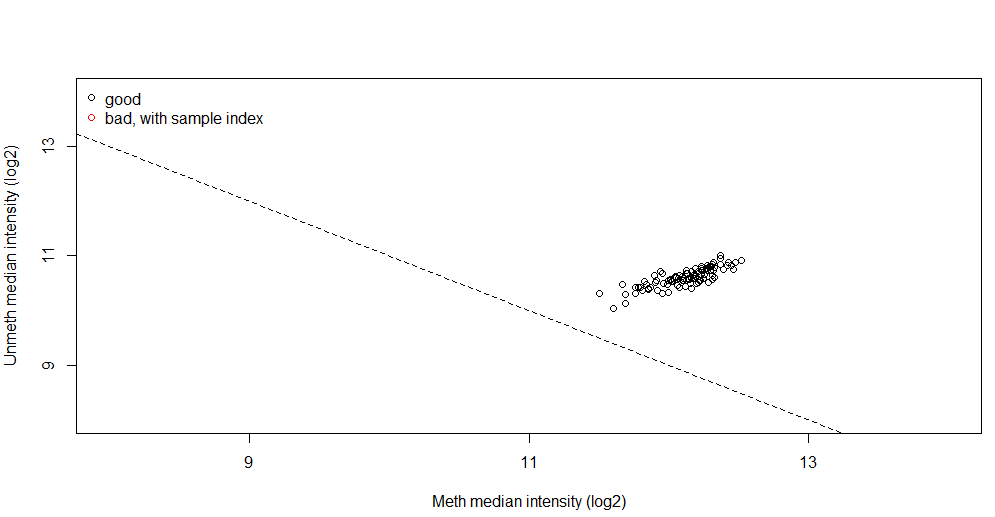
\includegraphics[width=90mm]{./11.png}
    \caption{
      The plot of quality control with getQC, addQC, and plotQC functions.
    }
  \end{center}
\end{figure}

PlotQC plot (Figure 7) demonstrates that bad samples do not exist in our
data set.

Comparison of methylation in density plots (Figure 8) indicates high
data quality because no notable deviations are visible from the rest of
the samples. Also significant alterations between different diagnosis
are not present.

\begin{figure}[!h]
  \begin{center}
    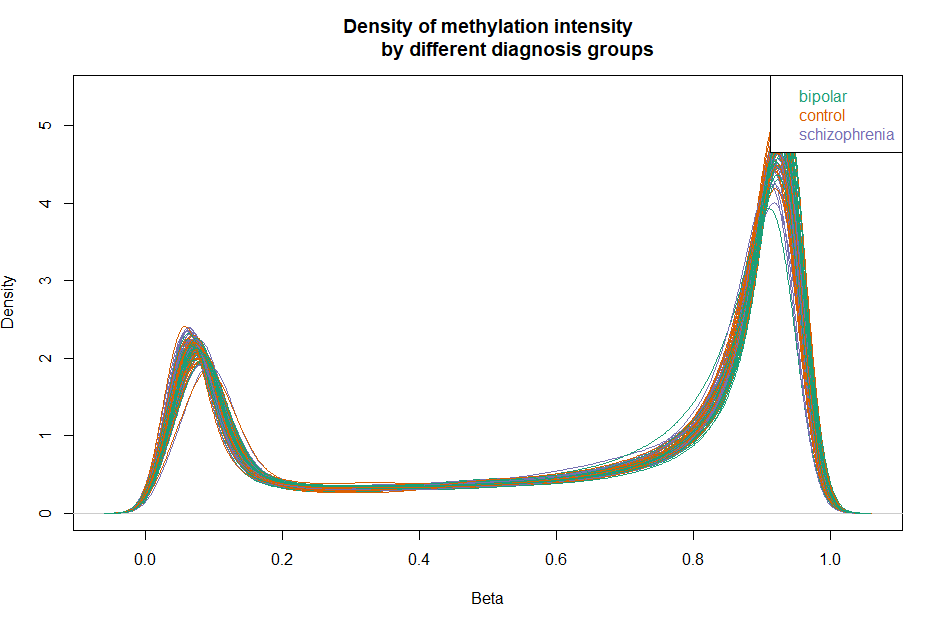
\includegraphics[width=75mm]{./12.png}
    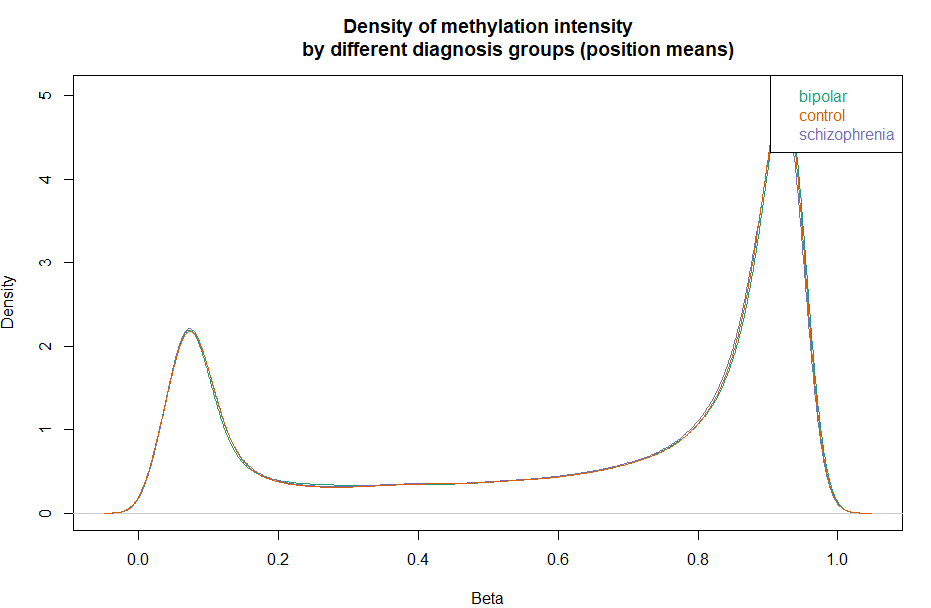
\includegraphics[width=75mm]{./13.png}
    \caption{
      The density plot of methylation intensity of each sample(left) and 
      density plot of all samples positions mean methylation intensity (right).
    }
  \end{center}
\end{figure}

\hypertarget{saving-data}{%
\subsection{Saving data}\label{saving-data}}

Data was saved into \emph{GSE112179\_clear.rds} file after the
processing.

\hypertarget{data-clustering}{%
\section{Data clustering}\label{data-clustering}}

For the second task it was required to perform data clustering.

Removing left-over samples from beta matrix

Calculation of distance matrix. \texttt{dist} function could not be used
due to `vector memory exhausted (limit reached?)' error message.

Data clustering was performed using \texttt{hclust} function with
\texttt{ward.d} linkage method. This method takes into account variance
of the clusters, thus it is said that it is the most eligible method for
quantitative data sets.

\begin{figure}[!h]
  \begin{center}
    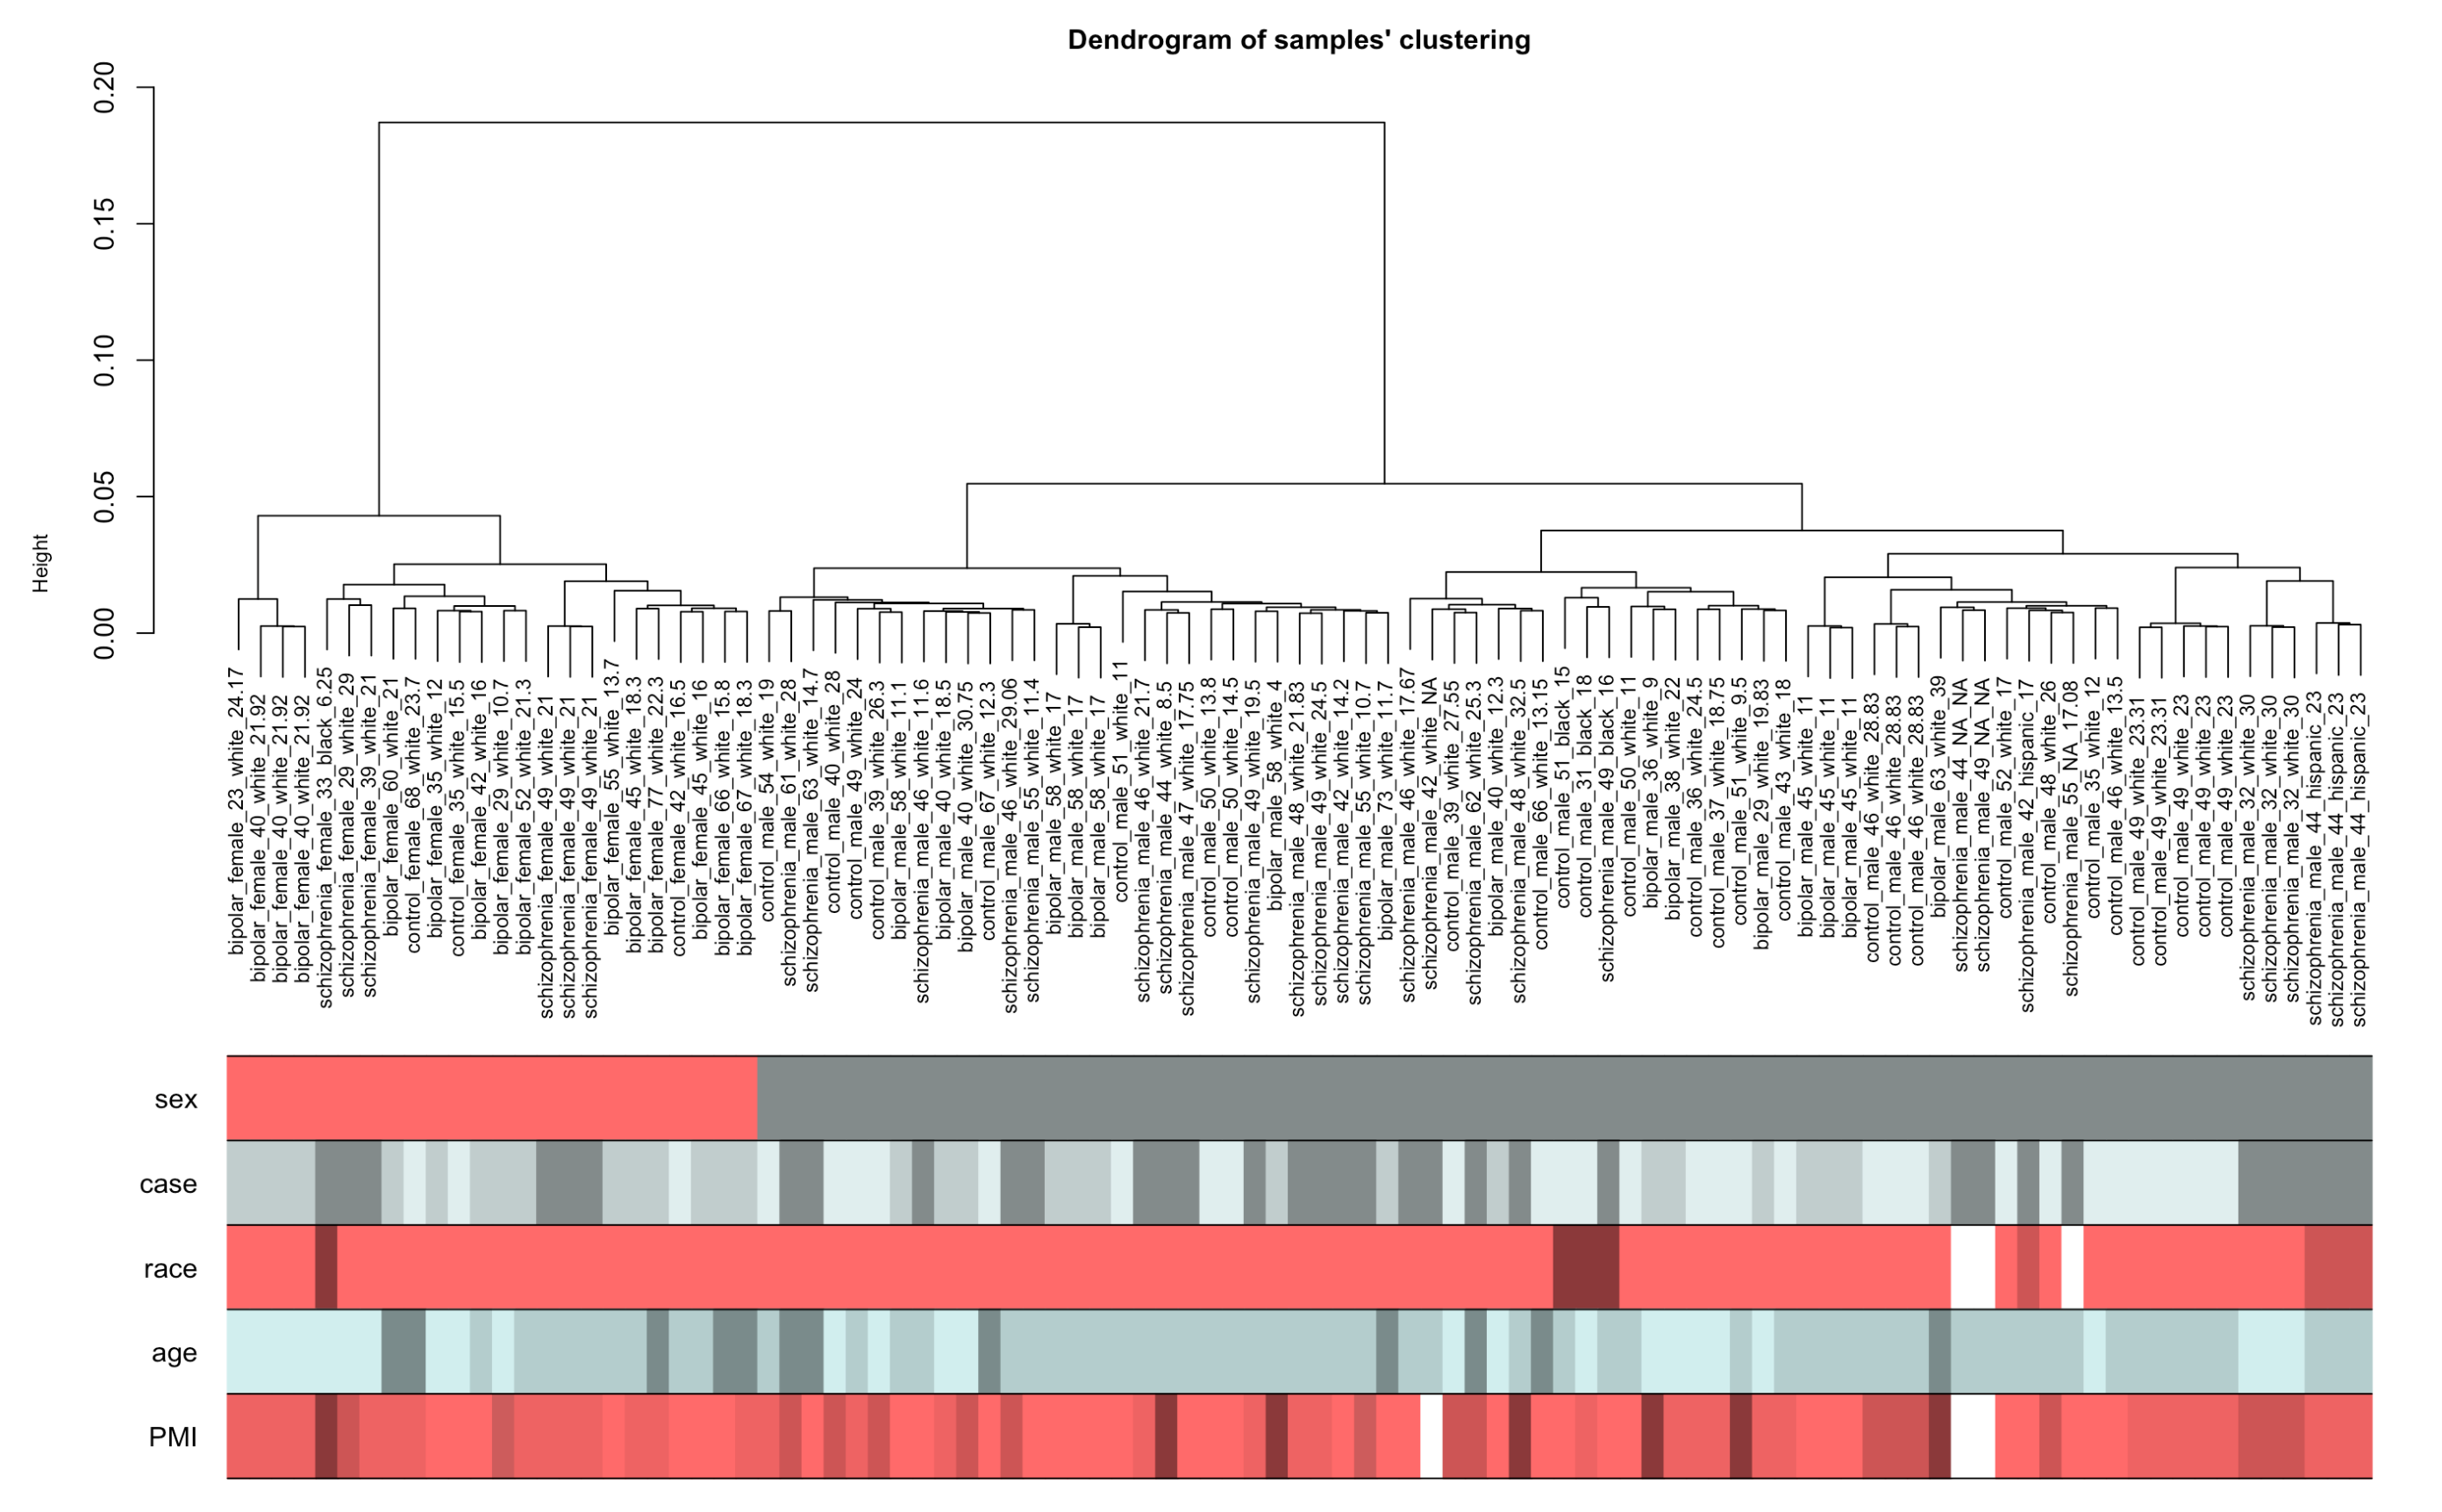
\includegraphics[width=150mm]{./14.png}
    \caption{
      The dendogram that shows three clusters after the hierarchical clustering
      using 1-cor() distance metric and Ward linkage method.
    }
  \end{center}
\end{figure}

The dendrogram (Figure 9) shows three distinguished groups after
clusterisation. It is worth noting that NA values are marked as white
color (such examples can be observed in race and post-mortal interval
colouring)

Clusters were analysed with the respect of sex, case, race, age, and
post-mortal interval groups. The main two clusters were distinguished
based on sex. Within these two main clusters, samples were clustered
into small case groups. The case groups are denoted by colours: dark,
medium, and light greenish gray.

The first group is overall composed of 24 samples. This collection
contains 15 samples of bipolar cases, 6 samples of schizophrenia, and 3
samples of control.

Second and third groups are separated from the first group.

The second group is made of 29 samples, of which 8 are control, 8 are
bipolar, and 13 are schizophrenia cases.

The third group has got 44 samples: 21 belong to control, 9 to bipolar,
and 15 to schizophrenia cases.

Regarding these clustering results, it could be stated that within each
of the clusters there is one dominant case. In the first cluster it is
bipolar, in the third - control, and in the second - schizophrenia.

The majority of samples had race `white' (marked as the lightest pink
colour). Race `hispanic' is marked with a medium pink colour, and race
`black' is marked with the darkest pink colour. Due to such imbalance,
clusterisation analysis in regards of `race' feature cannot give any
strong conclusions.

There are 3 age intervals that are noted with colours from lightest to
darkest greenish gray: 23-40, 41-58, 59-77. The biggest cluster of the
first age group can be observed within female samples. This cluster is
composed of bipolar and schizophrenia case samples. Another more
significant cluster can be observed within males of the middle age
group. This cluster is composed of all cases, however the majority of
cases are schizophrenic. The last age group is scattered in the whole
range of the dendogram (in all clusters of the tree).

The post-mortem interval colouring (from youngest to oldest brightness
in colour decreases) shows that most of the samples were collected
within 18 time units after death.

\hypertarget{heatmap-plotting}{%
\section{Heatmap plotting}\label{heatmap-plotting}}

The second part of the second task was to provide heatmaps for the most
varying positions in the data set. The variability of each position was
measured by calculating its variance within the samples.

\hypertarget{clocks-of-dna-modification}{%
\section{Clocks of DNA modification}\label{clocks-of-dna-modification}}

The third part of the second task requires to predict age of patients
from which the samples were taken and compare predictions with the real
data. Furthermore, the next step for the analysis is to check, whether
there is a significant difference of predicted age within each
experimental group.

Firstly, it was checked, which methylation clocks can be computed and
which cannot for the given data set if the threshold of 80\% of required
CpGs is set to compute each clock (Pelegı́-Sisó et al., 2021). The
threshold can be changed, however, the default one (80\%) was used in
this analysis.

\begin{center}
  \begin{tabular}{|l|r|}
      Clock & Missing CpGs (\%) \\
      \hline 
      Horvath & 5.1  \\
      Hannum & 11.3 \\
      Levine & 0.2 \\
      SkinHorvath & 0.0  \\
      PedBE & 0.0  \\
      WU & 3.6  \\
      TL & 0.0  \\
      BLUP & 0.5  \\
      EN & 0.0  \\
      \caption{
        Table of missing CpG positions for each clock
      }
  \end{tabular}
\end{center}

It was checked with \texttt{checkClocks} and \texttt{DNAmAge} functions
that the only clock which could not be computed for the given data set
was Bayesian Neural Network (BNN) (Alfonso \& Gonzalez, 2020)
(\texttt{DNAmAge} without age acceleration wrote NAs in the output).

\begin{figure}[!h]
  \begin{center}
    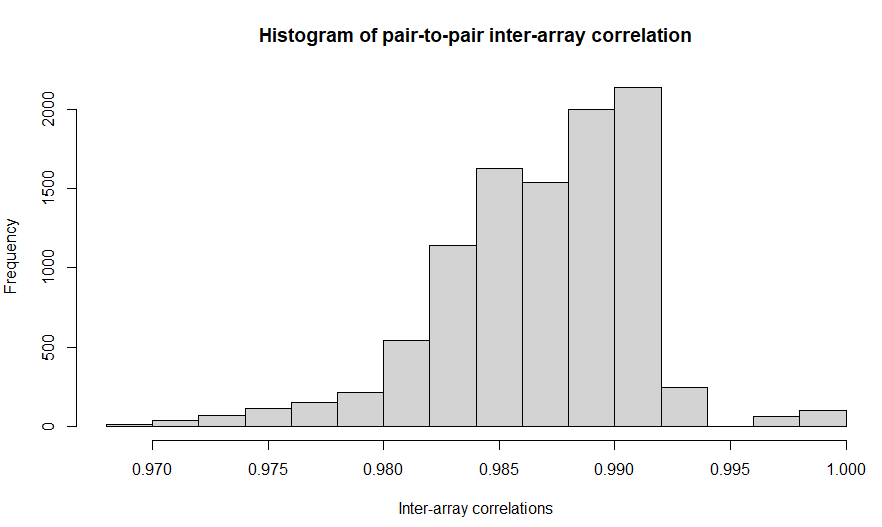
\includegraphics[width=15mm]{./1.png}
    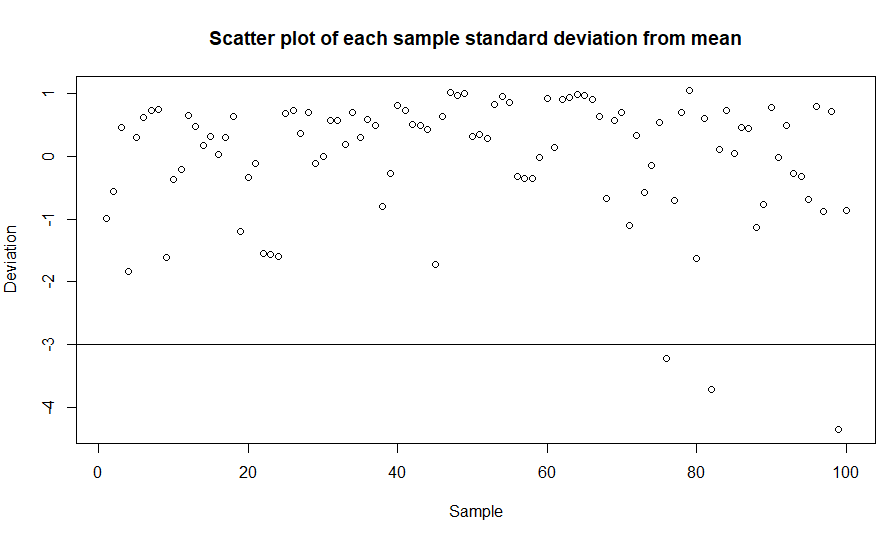
\includegraphics[width=15mm]{./2.png}
    \caption{
    Correlation between biological age predicted by methylation clocks and the 
    chronological age
    }
  \end{center}
\end{figure}

\hypertarget{checking-how-predicted-ages-differ-between-experimental-groups}{%
\subsection{Checking how predicted ages differ between experimental
groups}\label{checking-how-predicted-ages-differ-between-experimental-groups}}

The experimental groups of our research are control, bipolar, and
schizophrenia, therefore, predicted age values will be analysed with
regards of this sample grouping.

It was decided to run ANOVA tests for each methylation clock applied to
our data set.

\begin{itemize}
\item
  Data: difference between DNA methylation age and chronological age.
\item
  Test: ANOVA.
\item
  Hipotheses: \[H_0: \mu_1=\mu_2=\mu_3\]
  \[H_1: \exists i,j\in\{1,2,3\}: i\neq j, \mu_i \neq \mu_j\]
\item
  Significance level: \(\alpha=0.1\).
\item
  \(p\) value \(> \alpha \rightarrow H_0\) not rejected.
\end{itemize}

None of the ANOVA tests had p value lower than \(\alpha\), therefore
there are no differences in biological age between control, bipolar, and
schizophrenic sample groups.

EXTRA (try the flow with Euclidean distance)

\hypertarget{references}{%
\section*{References}\label{references}}
\addcontentsline{toc}{section}{References}

\hypertarget{refs}{}
\begin{CSLReferences}{1}{0}
\leavevmode\vadjust pre{\hypertarget{ref-alfonso2020bayesian}{}}%
Alfonso, G., \& Gonzalez, J. R. (2020). Bayesian neural networks for the
optimisation of biological clocks in humans. \emph{bioRxiv}.

\leavevmode\vadjust pre{\hypertarget{ref-fortin485512analysis}{}}%
Fortin, J.-P., \& Hansen, K. D. (n.d.). Analysis of 450k data using
minfi. \emph{Dim}, \emph{485512}, 6.

\leavevmode\vadjust pre{\hypertarget{ref-imatsentrix}{}}%
National Institutes of Health, N. C. I. at the. (n.d.). \emph{Sentrix®
BeadChip and BeadArray technology (illumina, inc.) \textbar{} innovative
molecular analysis technologies (IMAT)}.
\url{https://imat.cancer.gov/about-imat/outputs-and-achievements/individual-technologies-and-platforms/sentrix\%C2\%AE-beadchip-and}

\leavevmode\vadjust pre{\hypertarget{ref-pai2019differential}{}}%
Pai, S., Li, P., Killinger, B., Marshall, L., Jia, P., Liao, J.,
Petronis, A., Szabó, P. E., \& Labrie, V. (2019). Differential
methylation of enhancer at IGF2 is associated with abnormal dopamine
synthesis in major psychosis. \emph{Nature Communications},
\emph{10}(1), 1--12.

\leavevmode\vadjust pre{\hypertarget{ref-pelegi2021methylclock}{}}%
Pelegı́-Sisó, D., Prado, P. de, Ronkainen, J., Bustamante, M., \&
González, J. R. (2021). Methylclock: A bioconductor package to estimate
DNA methylation age. \emph{Bioinformatics}, \emph{37}(12), 1759--1760.

\end{CSLReferences}

\end{document}
